\documentclass{article}
\usepackage[utf8]{inputenc}
\usepackage{amsmath}
\usepackage{graphicx}
\usepackage{amssymb}
\usepackage{geometry}
\usepackage{alltt}
% \usepackage{subcaption}
\usepackage[shortlabels]{enumitem}
\usepackage{floatrow}
\usepackage{multirow}
\usepackage[utf8]{inputenc}
\usepackage[english]{babel}
\usepackage{hyperref}
\usepackage[backend=bibtex8]{biblatex}
\usepackage{listings}
\usepackage{xcolor}
%\usepackage{subfig}
\usepackage{subfigure}
\usepackage{blindtext}
\usepackage{amssymb}
\usepackage[ruled,vlined]{algorithm2e}
\usepackage{algorithm}
\usepackage{algorithmic}
\usepackage{booktabs}
\def\NoNumber#1{{\def\alglinenumber##1{}\State #1}\addtocounter{ALG@line}{-1}}
\usepackage{float}
\lstset { %
    frame=tb, % draw a frame at the top and bottom of the code block
    tabsize=4, % tab space width
    showstringspaces=false, % don't mark spaces in strings
    numbers=left, % display line numbers on the left
    commentstyle=\color{red}, % comment color
    keywordstyle=\color{blue}, % keyword color
    stringstyle=\color{green}, % string color
    breaklines=true % Fix margin stuff
}
\bibliography{references}

\title{GPU Accelerated Image Deblurring}
\author{Guy Bar, Armaan Kohli}
\date{\today}

\begin{document}
\maketitle
\tableofcontents
\newpage

\section{Problem Statement and Motivation}

In this project we measure and evaluate the benefits of using a graphics processing unit (GPU) over a central processing unit (CPU)
for an image blurring task. We also use this project as a means of understanding the basics of CUDA C/C++ and the Nvidia toolchain for GPU programming. 


\section{Introduction and Background}

Image blur is a common phenomena that occurs
for a variety of reasons. For example, one might observe image blur when they take a photograph while moving. With the rise of social media and photo-sharing applications, there has been a lot of interest in methods to improve image quality, such as deblurring. Image deblurring is also a common task in optical microscopy, where an image is often blurred along a single axis. 

Due to the varied use cases,
image blurring can be caused in different ways.
A blurry image $B$ is usually modeled as a convolution
between an image, $I$, and a blurring kernel $K$:
\begin{eqnarray}
    B = I * K
\end{eqnarray}
Often times the $B$ and $K$ are known and therefore the
process of image deblurring usually boils down to a 
de-convolution to compute $I$.
In our case, however, $K$ is not know and so we have to
compute both $K$ and $I$ in what is known as blind de-convolution.
More information can be found in section \ref{section:algo}.

The main focus of our project is to quantify the 
differences between running our algorithm on a CPU and a GPU. GPUs are designed to parallelize computational tasks, so performing operations such as multiplication, addition and convolution between images on a GPU can be much faster than the same operations performed on a CPU.

Armaan Kohli managed the CPU code and the testing, Guy Bar handled the GPU code and algorithm implementation. 

\clearpage
\subsection{Image Deblurring Algorithms} \label{section:algo}

There are two main ways to deblur images, non-blind and blind methods. Non-blind methods are simpler but make the strong assumption that we know exactly how the image was blurred. In other words, we know the function $K$, sometimes referred to as a point-spread function (PSF), that took the non-blurred target image $I$ and generated the image we need to process, $B$ via convolution.  If we know the functional form of the $K$, then we can perform a deconovlution operation to recover the original image $I$ from it's blurred counterpart $B$. 

However, it is fairly rare that we know the function $K$. As an example, in our application we don't have knowledge of the PSF. Therefore we must resort to using a blind method for deblurring. Blind algorithms make no assumptions about the PSF and can thus  be used in settings where the PSF is unknown. 

We implement two different kinds of blind image deblurring algorithms. First, there are methods that attempt to estimate the PSF, such as the so-called Lucy-Richardson Algorithm. 
\begin{algorithm}
\caption{Lucy-Richardson}
\begin{algorithmic} 
\REQUIRE $B$, \texttt{numIter}
    \STATE $\hat{I} \leftarrow B$
    \STATE $\hat{K} \leftarrow  \mathcal{N}(0, I)$
    \STATE $i \leftarrow 0$
    \WHILE{$i < $ \texttt{numIter}}
          \STATE $\hat{K} _{i+1} = \left[ \left(\frac{B}{\hat{K}_i * \hat{I}_i}      \right) * \hat{I}_i \right]\hat{K}_i $ //update PSF estimate 
           \STATE $\hat{I} _{i+1} = \left[ \left(\frac{B}{\hat{I}_i * \hat{K}_i}      \right) * \hat{K}_i \right]\hat{I}_i $ //  update Image estimate
        % \STATE $\hat{c} \leftarrow \hat{u} \circledast P$
        % \STATE \texttt{relBlur} $\leftarrow d / \hat{c}$
        % \STATE  \texttt{err} $\leftarrow $ \texttt{relBlur} $ \circledast$ $\hat{P}$
        % \STATE $\hat{u} \leftarrow \hat{u}$ $*$ \texttt{err}
        \STATE $i \leftarrow i + 1$
    \ENDWHILE
    \RETURN $\hat{I}$
\end{algorithmic}
\end{algorithm}\\
This algorithm performs an iterative estimate of the point spread function, $\hat{K}$, and estimates the deblurred image $\hat{I}$. As presented above, we perform one PSF estimate per image estimate. However, in practice, you can perform repeated estimates of the PSF before updating the image \cite{LRalgo}.

Another class of algorithms are methods that completely ignore the existence of the PSF and simply attempt to restore salient features that blurring tends to distort, such as image borders. One such method is the application of a simple sharpening filer. This algorithm only requires a single convolution, between the image and a pre-determined kernel function. One such example of a sharpening kernel is:
\begin{equation}
    K = 
\begin{pmatrix}
0 & -1 & 0 \\
-1 & 5 & -1 \\
0 & -1 & 0
\end{pmatrix}
\end{equation}
\begin{algorithm}
\caption{Sharpening Filter}
\begin{algorithmic} 
\REQUIRE $B$, $K$
    \STATE $\hat{I} = B * K$
    \RETURN $\hat{I}$
\end{algorithmic}
\end{algorithm}\\
The advantage of the Lucy-Richardson algorithm is that you can potentially recover the deblurred image almost exactly, at the cost of more compute time, since it is an iterative algorithm. The sharpening filter, on the other hand, can at the best case only restore borders and edges, but requires much less time to compute. 


\subsection{CUDA}
The Compute Unified Device Architecture, or CUDA, is an API created by Nvidia to develop software that utilizes Nvidia's GPU resources. There is a C/C++ implementaion that can be compiled using Nvidia's proprietary nvcc compiler.

The particular computer we used in our project is the Nvidia Jetson Nano. The Jetson Nano includes both a CPU and a GPU, allowing us to run our CPU and GPU implementations sequentially and compare our results.


\section{Implementation}
In order to compare the performance of our deblurring algorithms, we implement them on both a conventional CPU architecture and on a GPU. 

\subsection{Image Coding}
Before any image processesing tasks can be done, we must first be able to load an image into memory. This is a surprisingly complex task. Images aren't typically stored as arrays you can easily manipulate, they are first encoded, for example as a \texttt{.png} or \texttt{.jpg} file, as a form of data compression. Thus, in order to manipulate any sort of image in our program, we must first decode the image. Then, after performing image deblurring, we must encode our array back to a suitable image format. We choose to work with only \texttt{.png} files. This meant that we had to convert any \texttt{.jpg} into \texttt{.png} files. We did this using the \texttt{convert} command line tool, as part of the \texttt{ImageMagick} suite, often included standard as part of many *nix operating systems. In order to encode and decode \texttt{.png} images, we used the \texttt{libpng} library and a \texttt{C++} wrapper for it called \texttt{png++}. \texttt{libpng} is the official PNG reference library for the C programming language, and has been in use for over 23 years. We opted to use an open-source PNG library, since developing our own PNG codec for this project would not have been a realistic endeavour. 

Using \texttt{libpng}, we can decode images into our custom Image data structure and then once the image deblurring algorithm has finished we can encode our image back to a \texttt{.png} file. 

\subsection{Algorithm} \label{section:our_Algo}
Although at first we attempted to implement the blind lucy-richardson algorithm described in \cite{LRalgo}, we ran into complexity problems rather quickly when we realized that the PSF and image had to be the same size. Taking the NASA Earth image as an example, a convolution between two 960x960 arrays was simply not computationally feasible. As such, we turned our attention to the regular Lucy-Richardson algorithm and the sharpening filter.

We found experimentally that neither Lucy-Richardson or the sharpening filter worked well on their own. After a few iterations, the estimate of the PSF from Lucy-Richardson was inaccurate and led to noisy images with ringing artifacts, and alone, the sharpening filter didn't do much to improve image quality. So, we developed our own, hybrid algorithm for image deblurring, presented below. 
\begin{algorithm}
\caption{Hybrid Deblurring Algorithm}
\begin{algorithmic} 
\REQUIRE $B$, $K$
    \STATE $\hat{I} \leftarrow B$
    \STATE $\hat{K} \leftarrow  \mathcal{N}(0, I)$
    \STATE $i \leftarrow 0$
    \WHILE{$i < $ \texttt{1}} 
          \STATE // Lucy-Richardson Deconvolution 
          \STATE $\hat{K} _{i+1} = \left[ \left(\frac{B}{\hat{K}_i * \hat{I}_i}      \right) * \hat{I}_i \right]\hat{K}_i $  
           \STATE $\hat{I} _{i+1} = \left[ \left(\frac{B}{\hat{I}_i * \hat{K}_i}      \right) * \hat{K}_i \right]\hat{I}_i $ 
        % \STATE $\hat{c} \leftarrow \hat{u} \circledast P$
        % \STATE \texttt{relBlur} $\leftarrow d / \hat{c}$
        % \STATE  \texttt{err} $\leftarrow $ \texttt{relBlur} $ \circledast$ $\hat{P}$
        % \STATE $\hat{u} \leftarrow \hat{u}$ $*$ \texttt{err}
        \STATE $i \leftarrow i + 1$
    \ENDWHILE
    \STATE $\hat{I} = \hat{I}* K$ // Apply sharpening filter
    \RETURN $\hat{I}$
\end{algorithmic}
\end{algorithm}\\
This algorithm combines Lucy-Richardson deconvolution and the sharpening filter. First, we compute one Lucy-Richardson iteration to obtain a rough estimate of the PSF and the underlying, unblurred image. We then apply a sharpening filter to improve the quality of edges. This is the algorithm that yields the best results in terms of image quality when run on the CPU. As such it is the algorithm we chose to use and implement on the GPU. 


\subsection{CPU Implementation}
The CPU implementation of the deblurring algorithms are fairly straight forward. First, we read in two images, the un-blurred image and the blurry image. We then run the algorithm to generate a deblurred image. We then compute the PSNR of our deblurred image. We present pseudo-code for the worflow below:
\begin{verbatim}
    Image blurryImage = imread(`blurry_image.png')
    Image unblurredImage = imread(`unblurred_image.png')
    timer_start()
    Image deblurredImage = deblur(blurryImage)
    timer_end()
    imwrite(deblurredImage, `deblurred_image.png')
    PSNR = psnr(deblurredImage, unblurredImage)
\end{verbatim}{}
The \texttt{deblur} function either calls a function to perform Lucy-Richardson blind deconvolution or a sharpening filter, as discussed prior. 

  

\subsection{GPU Implementation}
The GPU implementation of the deblurring algorithms start in a similar way. First, we load the un-blurred and blurred images into the host device memory. Next, we allocate all of the memory on the target device required for the particular algorithm to run. 

Next, we call a sequence of kernel functions, each representing a single mathematical operation in the deblurring algorithm.
An important feature in our kernel functions is their image size invariance. Our kernel functions were designed from the ground up to handle arbitrarily sized images.
We accomplished this by using a common structure for all our kernel functions: a for-loop that allows each thread in each block to start at a unique and consecutive index in the image and then at each for-loop iteration increase by a multiple of the total number of threads in the grid. Our kernel function structure looks like so:
\begin{alltt}   
    const int start_idx = blockDim.x * blockIdx.x + threadIdx.x;
    const int stride    = blockDim.x * gridDim.x;
    const int max_val   = 3*H*W;
    
    for (int idx = start_idx; idx < max_val; idx += stride) 
    \{
        \vdots
    \}
\end{alltt}{}

Each kernel function is executed sequentially in the GPU, with the GPU waiting for the full kernel function implementation to finish before beginning the executing of the next one.
This, along with the structure shown above, led us to conclude that the optimal number of threads per block and number of blocks per grid should theoretically be as large as possible. As such, we chose to make them 1024 and 131070 respectively. It is interesting to note, however, that we experimented with different values for these variables and found no significant differences. Perhaps this is a consequence of a large number of for-loop iterations each thread is required to execute. Nevertheless, we decided to stick with the theoretically optimal values.


\subsection{Performance Metrics}
To evaluate the performance of our algorithms, we compare the time it takes to perform the deblurring task and the quality of the resultant image. In addition to the provided earth image, we also generated our own dataset to evaluate the performance of our algorithms on a variety of images. We generated the dataset using using a simple \texttt{MATLAB} script to blur several different images using a Gaussian filter. 

\subsubsection{Run Time}
We used the built-in tools in both C++ and CUDA to build timing metrics. To measure CPU performance, we used the \texttt{std::chrono} library to measure the execution time of the algorithm.  On the GPU side, we used several functions built into CUDA to perform timing analysis \cite{gputime}. In order to perform operations on the GPU, in addition to the actual algorithm itself, you first need to allocate memory and move data from the host to the target device, as part of I/O operations. I/O operations are often a significant  bottleneck for GPUs and so it is important that our GPU timing metric account for them. Even if the core algorithm on the GPU is faster, if I/O operations take up too much time it might be more practical to use a CPU implementation. 

\subsubsection{Image Quality}
We measure the quality of the deblurred image by a conventional image quality metric, the peak signal-to-noise ratio (PSNR). The formula for PSNR is calculated as:
\begin{equation}
\begin{align} 
PSNR = 10log_{10}\left(\frac{MAX_I^2}{MSE} \right) \\
MSE = \frac{1}{n^2}\sum_{i=0}^{n-1} \sum_{j=0}^{n-1} \left(I[i,j]- \hat{I}[i,j]\right)^2
\end{align}
\end{equation}
It is, in effect, a measure of the mean-squared error between the deblurred image, and the original, unblurred image. $MAX_I$ indicates the maximum value for that particular image representation. For example, an image represented in RGB values will have $MAX_I = 255$. PSNR is reported in units of decibels dB and is a standard metric of image quality. 

\section{Results and Discussion} 
First, we ran the algorithm on the NASA Earth dataset.
The original and blurry images can be seen in figure \ref{fig:NASA_original} and figure \ref{fig:NASA_blurry} respectfully.
As mentioned in section \ref{section:our_Algo}, we began our experimentation with the regular Lucy-Richardson and sharpening filters separately. Doing so saw an improved PSNR score as compared to the blurry image, however the image itself did not look significantly better— many of its edges got highlighted in unnatural colors. The results of the regular Lucy-Richardson algorithm can be seen in figure \ref{fig:NASA_lucyRich}.

Hoping to do better, we combined the lucy-richardson and sharpening filters into our hybrid algorithm. The hybrid algorithm achieved a significantly better PSNR and its result can be seen in \ref{fig:NASA_hybrid}.
Most importantly to this project, the performance increase when taking advantage of the Jetson Nano's GPU were significant. We were able to decrease our runtime by orders of magnitude. More information can be found in tables \ref{tab:runtime-nasa} and \ref{tab:psnr-nasa}.

Encouraged by the NASA Earth dataset result, we ran the hybrid algorithm on several other images that were blurred by us using a gaussian filter in \texttt{MATLAB}. Our results show comparable runtime improvements to the NASA image and can be found in table \ref{tab:runtime-dataset}. However, we were not able to observe improvements in PSNR across our custom dataset.

\begin{table}[htp]
\caption{Comparing runtime performance of algorithms optimized for CPU and GPU on the NASA Earth dataset}
\label{tab:runtime-nasa}
\begin{tabular}{ll}
\hline
\multicolumn{2}{c}{Runtime Comparisons - NASA Earth Dataset} \\ \hline
\multicolumn{1}{l|}{\begin{tabular}[c]{@{}l@{}}CPU\\ Time Elapsed  \end{tabular}} & 5681.368 (ms) \\ \hline
\multicolumn{1}{l|}{\begin{tabular}[c]{@{}l@{}}GPU\\ Time Elapsed  \end{tabular}} &  602.48 (ms) \\ \hline
\multicolumn{2}{c}{\textbf{843\% Improvement}} \\ \hline

\end{tabular}
\end{table}

\begin{table}[htp]
\caption{Evaluating improvements in image quality offered by our deblurring algorithm}
\label{tab:psnr-nasa}
\begin{tabular}{ll}
\hline
\multicolumn{2}{c}{PSNR - NASA Earth Dataset} \\ \hline
\multicolumn{1}{l|}{Blurry Image} & 17.041dB \\ \hline
\multicolumn{1}{l|}{Hybrid Deblurring Algorithm} & 17.162dB \\ \hline
\multicolumn{2}{c}{\textbf{0.673\% Improvement}}
\end{tabular}
\end{table}

\begin{table}[htp]
\caption{Average runtime performance for our custom dataset}
\label{tab:runtime-dataset}
\begin{tabular}{ll}
\hline
\multicolumn{2}{c}{Runtime Comparisons - Custom Dataset} \\ \hline
\multicolumn{1}{l|}{\begin{tabular}[c]{@{}l@{}}CPU\\ Avg. Time Elapsed\end{tabular}} & 4547.537 ms \\ \hline
\multicolumn{1}{l|}{\begin{tabular}[c]{@{}l@{}}GPU\\ Avg. Time Elapsed\end{tabular}} &  649.070 ms\\ \hline
\multicolumn{2}{c}{\textbf{ 600.62\% Improvement}}
\end{tabular}
\end{table}
% table comparing runtimes on CPU and GPU for earth dataset
% table comparing PSNR for earth dataset
% show images of earth 
% should probably generate our own dataset, compare results on that as well
\clearpage
\begin{figure*}[!htp]
    \begin{center}
        \subfigure[Original Image]{
        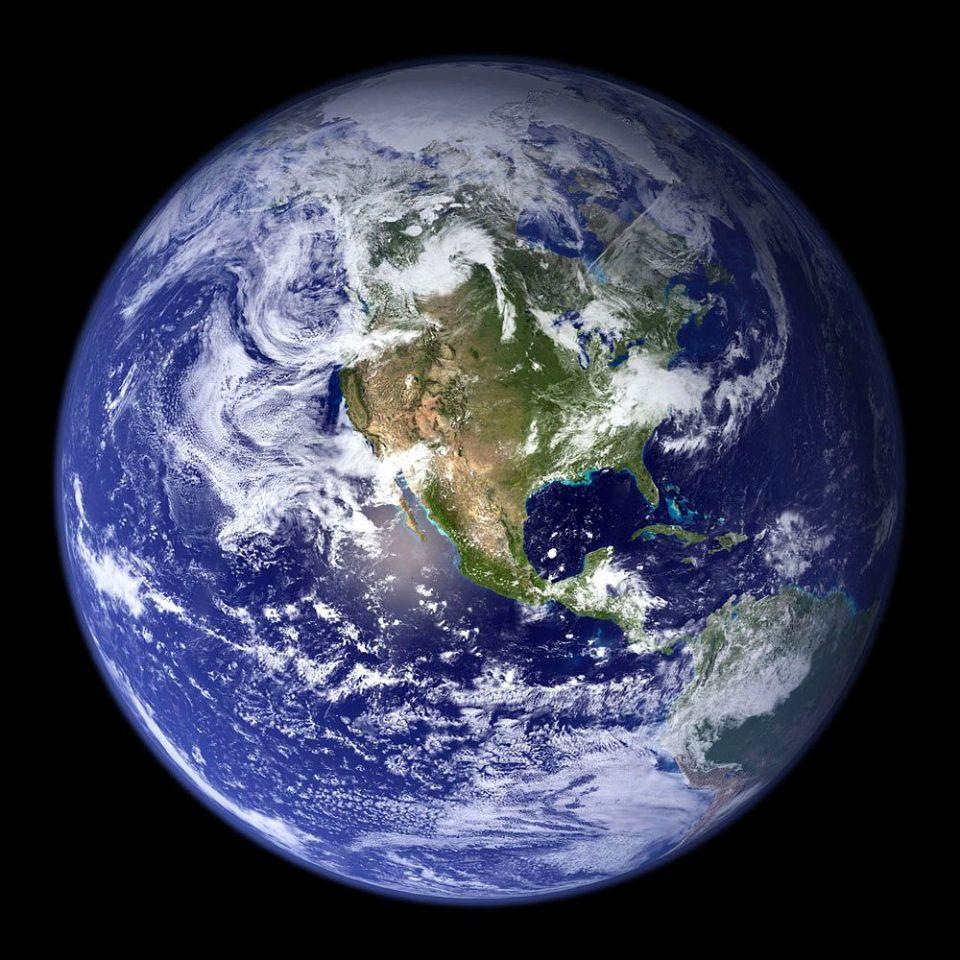
\includegraphics[width=2.8in]{figures/nasa_original.png}
        \label{fig:NASA_original}}
        \subfigure[Blurry Image]{
        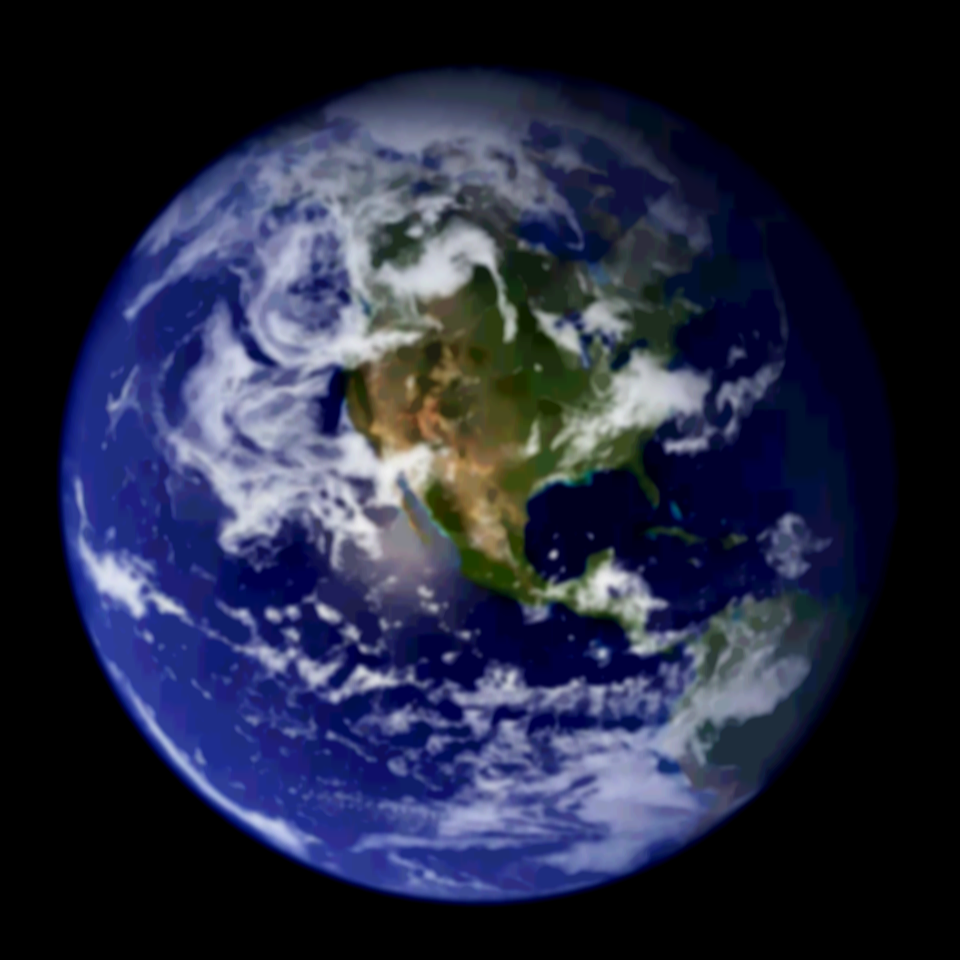
\includegraphics[width=2.8in]{figures/nasa_blurry.png}
        \label{fig:NASA_blurry}}
        \subfigure[Regular Lucy-Richardson Result]{
        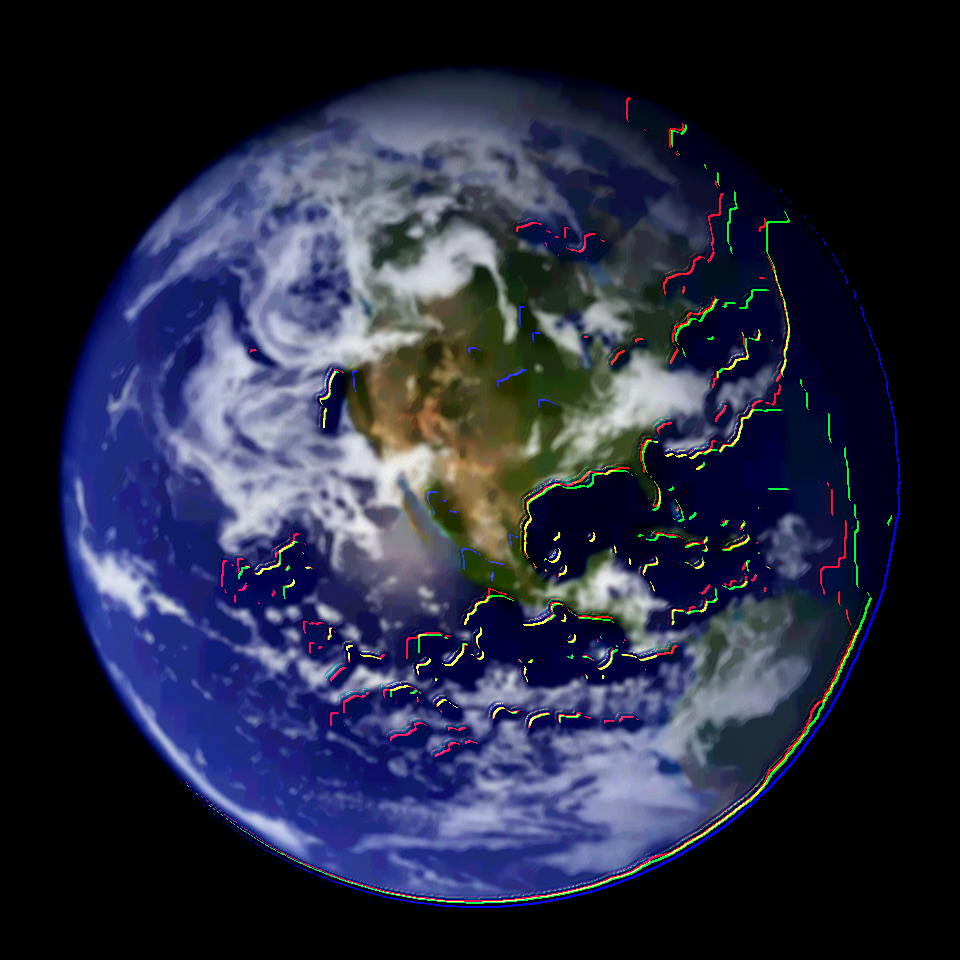
\includegraphics[width=2.8in]{figures/nasa_lucyRich.png}
        \label{fig:NASA_lucyRich}}
        \subfigure[Hybrid Algorithm Result]{
        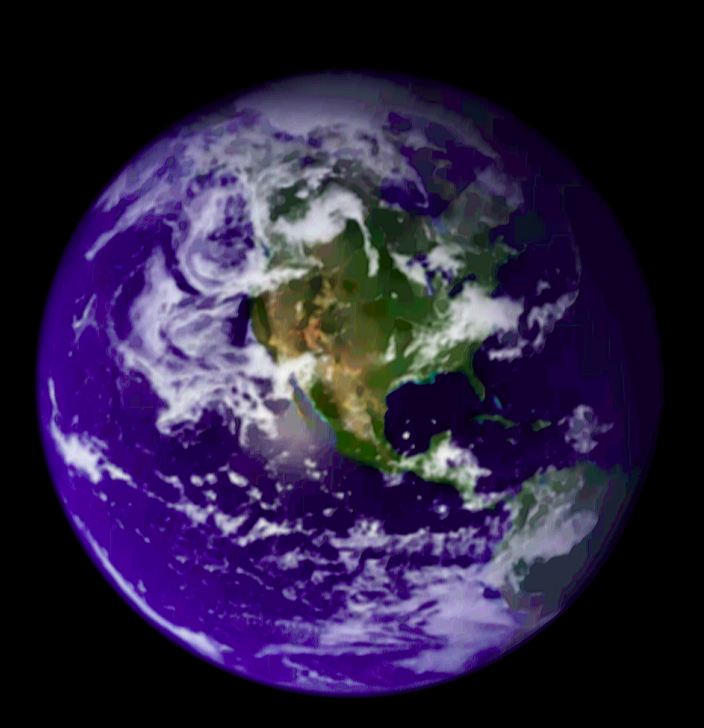
\includegraphics[width=2.8in]{figures/nasa_hybrid.png}
        \label{fig:NASA_hybrid}}
    \end{center}
\end{figure*}
\clearpage
\section{Conclusion}

In this project, we have successfully parallelized image processing algorithms using a GPU in order to improve the run-time performance. We were able to develop performance metrics to demonstrate the effectiveness of our GPU implementation. We also learned about CUDA C/C++ and the Nvidia toolchain for the Nvidia Jetson Nano. 

\printbibliography

\clearpage
\section{Appendix A: Instructions}

For the C libpng library and its C++ wrapper extension, png++, to work as intended, they first need to be installed. These should already be installed on the Jetson Nano, but you can also install the libraries manually as follows:
\begin{verbatim}
sudo apt-get install libpng-dev

wget download.savannah.nongnu.org/releases/pngpp/png++-0.2.9.tar.gz
sudo tar -zxf png++-0.2.9.tar.gz -C /usr/src
cd /usr/src/png++00.2.9
make
make install
\end{verbatim}
\texttt{libpng} is not available in the repos provided on the machine used to cross compile, since the operating system version is outdated. Thus, in order to run the program, you must \texttt{make} it directly on the Jetson Nano. 

After setup, to install the project, clone the repo into your directory of choice and go into the project directory

\begin{verbatim}
git clone https://github.com/armaank/cuda-deblur.git
cd cuda-deblur
\end{verbatim}

Now you can run the CPU and/or GPU implementation. 
To do so, go to the CPU and/or GPU directories, and call \texttt{make} followed by the executable. 
The executable takes in 3 arguments: the blurry image, the image output file name, and the original image. 
For example, to make the GPU code:
\begin{verbatim}
cd gpu
make
./gpu_deblur.out BLURRED_IMAGE OUTPUT_IMAGE_NAME ORIGINAL_IMAGE
\end{verbatim}
Likewise, to make the CPU code:
\begin{verbatim}
cd cpu
make
./cpu_deblur.out BLURRED_IMAGE OUTPUT_IMAGE_NAME ORIGINAL_IMAGE
\end{verbatim}
In order to compute and store logs of the results for the entire image dataset, you can use one of our provided `benchmark` scripts. 
For example, to benchmark the CPU code:
\begin{verbatim}
sh 
cd cpu
make
sh cpu_benchmark.sh
    \end{verbatim}
Likewise, to benchmark the GPU code:
\begin{verbatim}
cd gpu
make
sh gpu_benchmark.sh
\end{verbatim}

These will store statistics and output images into \texttt{*pu/output/benchmarks`}

% For the libpng library and its C++ wrapper extension, png++, to work as intended, they first need to be installed. Both the library and wrapper are installed on the Jetson Nano, but for reference, you can install manually as such:
% \begin{verbatim}
%     sudo apt-get install libpng-dev
    
%     wget download.savannah.nongnu.org/releases/pngpp/png++-0.2.9.tar.gz
%     sudo tar -zxf png++-0.2.9.tar.gz -C /usr/src
%     cd /usr/src/png++00.2.9
%     make
%     make install
% \end{verbatim}

% Now we can run the CPU and/or GPU implementation. 
% To do so, go to the CPU and/or GPU directory respectively, and call \texttt{make} followed by the executable. The executable takes in 3 arguments: the blurry image, the image output file name, and the original image. 
% This all looks like the following (when inside either the CPU or GPU directories):
% \begin{verbatim}
%     make
%     ./gpu_deblur.out ../data/nasaEarthBlurry.png outputImage ../data/nasaEarthOriginal.png
% \end{verbatim}
\clearpage
\section{Appendix B: Select Results from Custom Dataset}
We present select results from our custom dataset below.
\begin{figure*}[!htp]
    \begin{center}
        \subfigure[Original Image.\\ A lovely hydrangea]{
        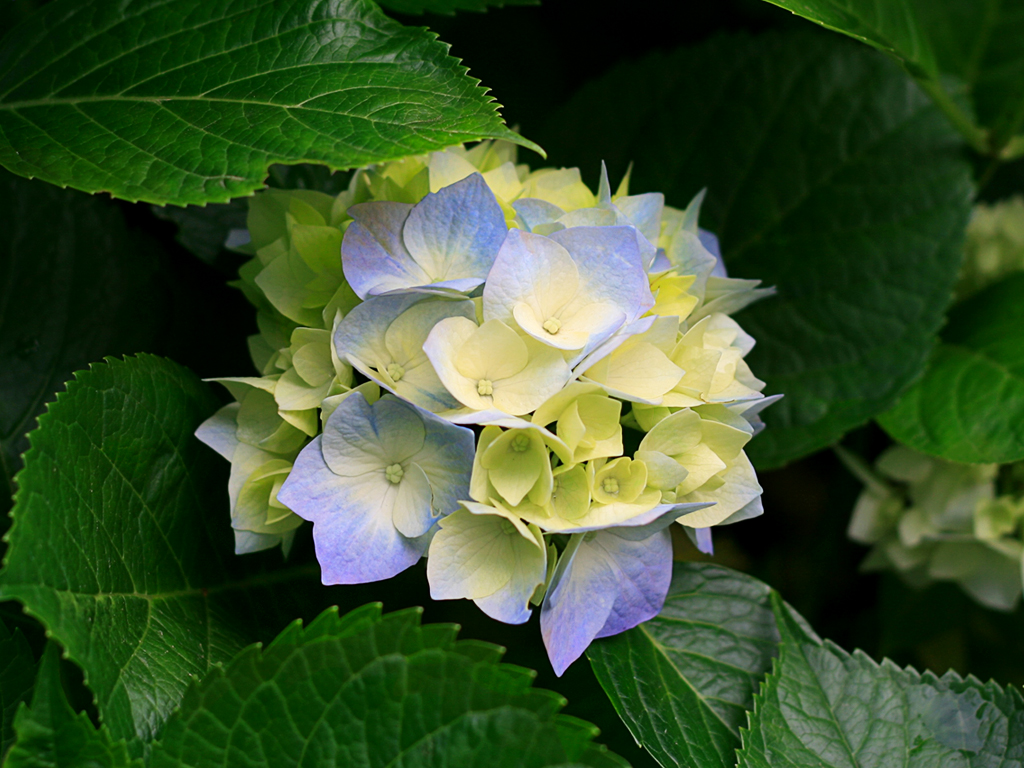
\includegraphics[width=1.6in]{figures/hydra.png}
        \label{fig:hyrda}}
        \subfigure[Blurry Image]{
        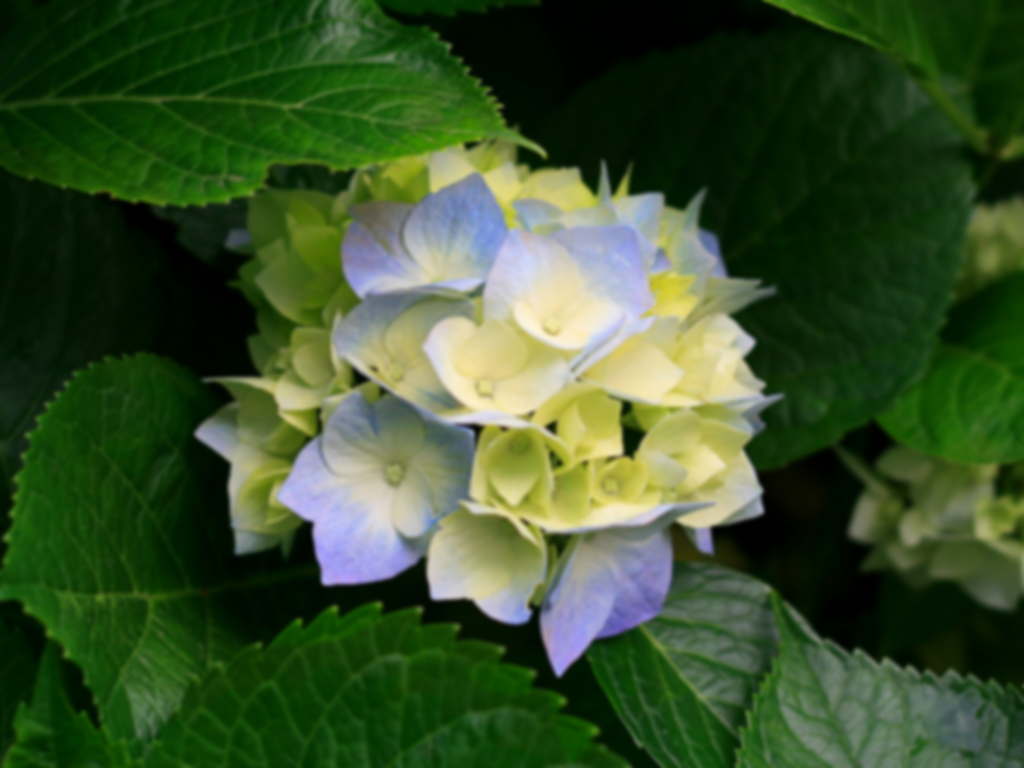
\includegraphics[width=1.6in]{figures/hydra_blurry.png}
        \label{fig:hyra_blurry}}
        \subfigure[Hybrid Algorithm Result]{
        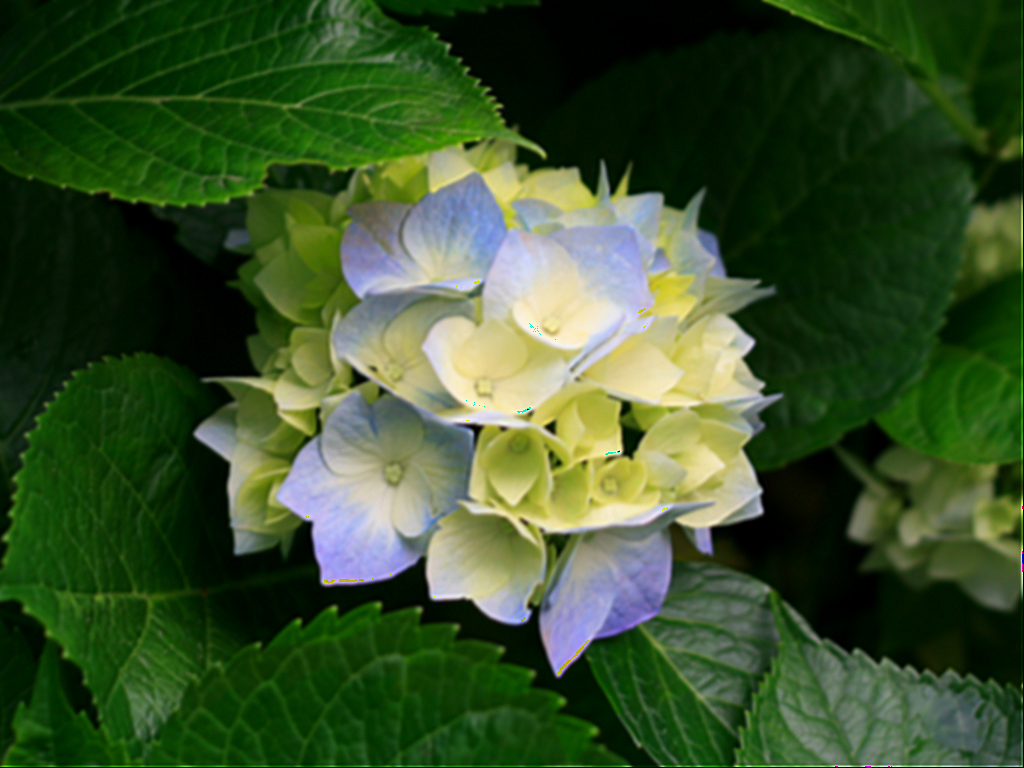
\includegraphics[width=1.6in]{figures/hydra_deblur.png}
        \label{fig:hydra_deblur}}
    \end{center}
\end{figure*}

\begin{figure*}[!htp]
    \begin{center}
        \subfigure[Original Image.\\ A picturesque image of the Scottish country side.]{
        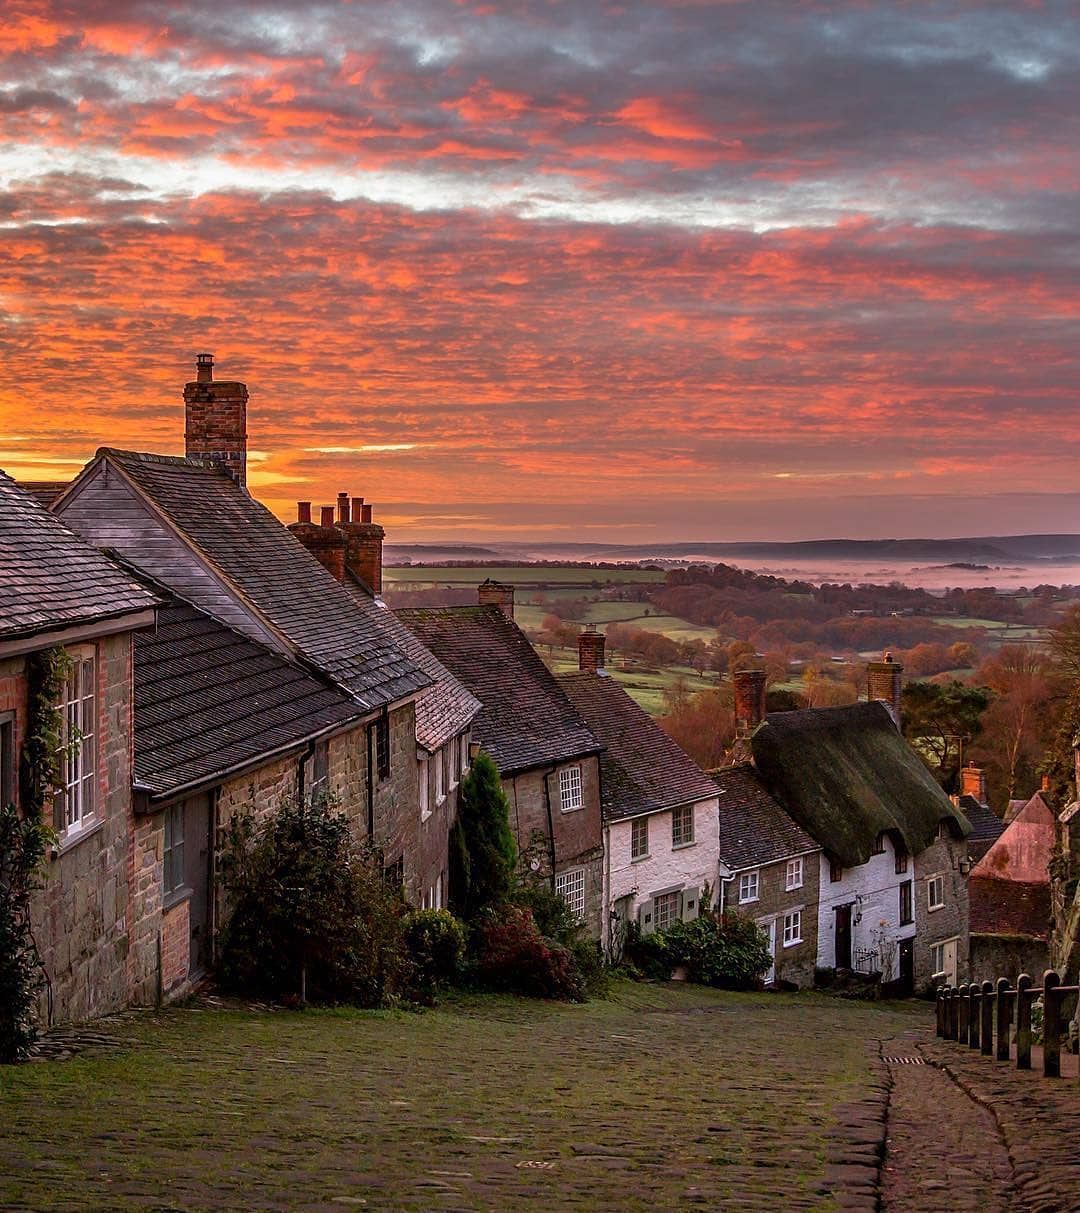
\includegraphics[width=1.6in]{figures/homes.png}
        \label{fig:hyrda}}
        \subfigure[Blurry Image]{
        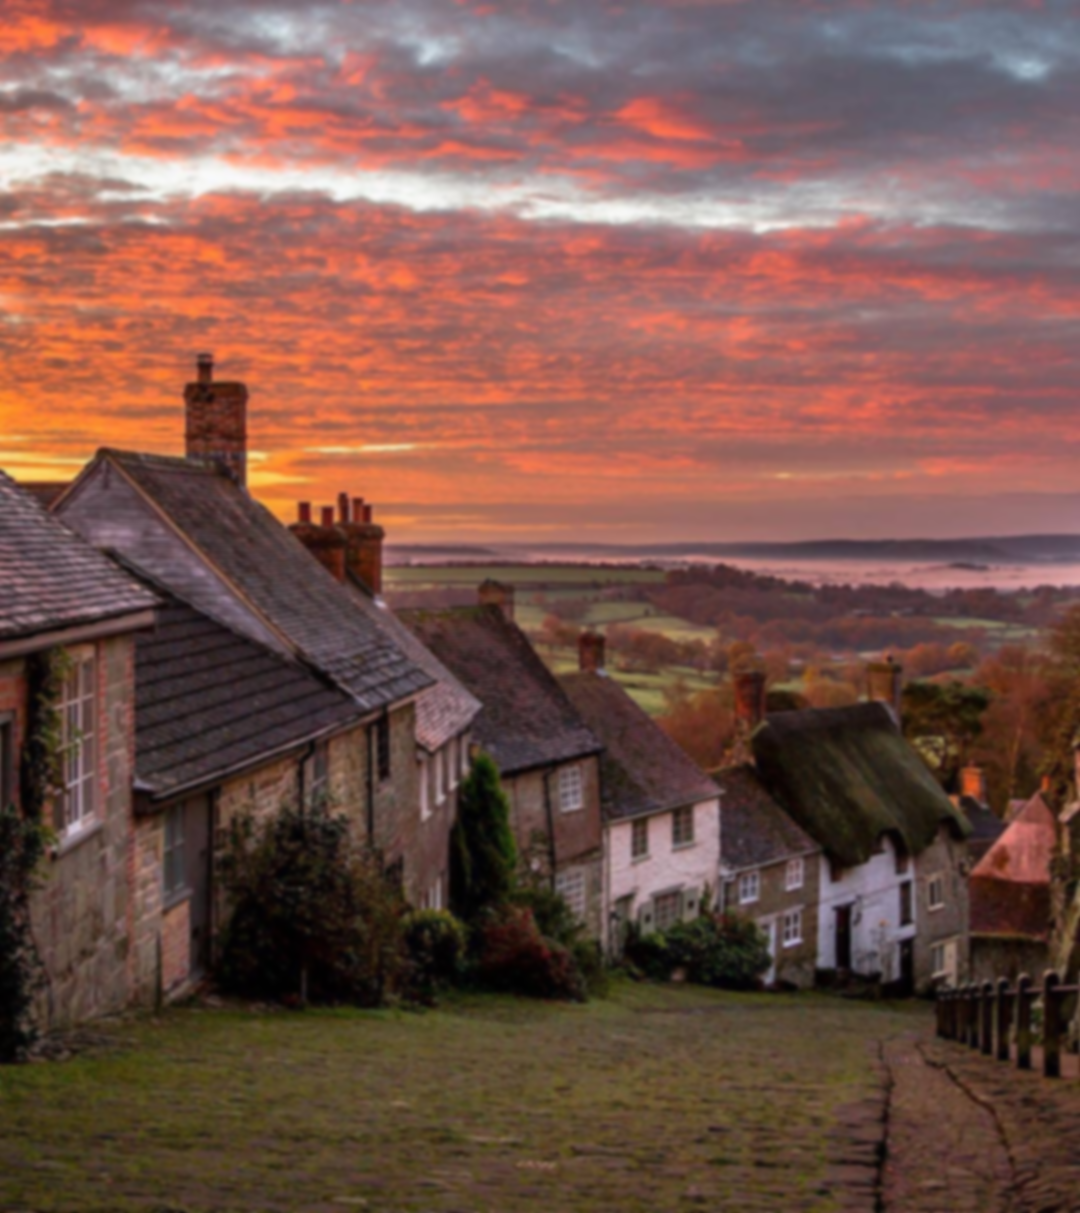
\includegraphics[width=1.6in]{figures/homes_blurry.png}
        \label{fig:hyra_blurry}}
        \subfigure[Hybrid Algorithm Result]{
        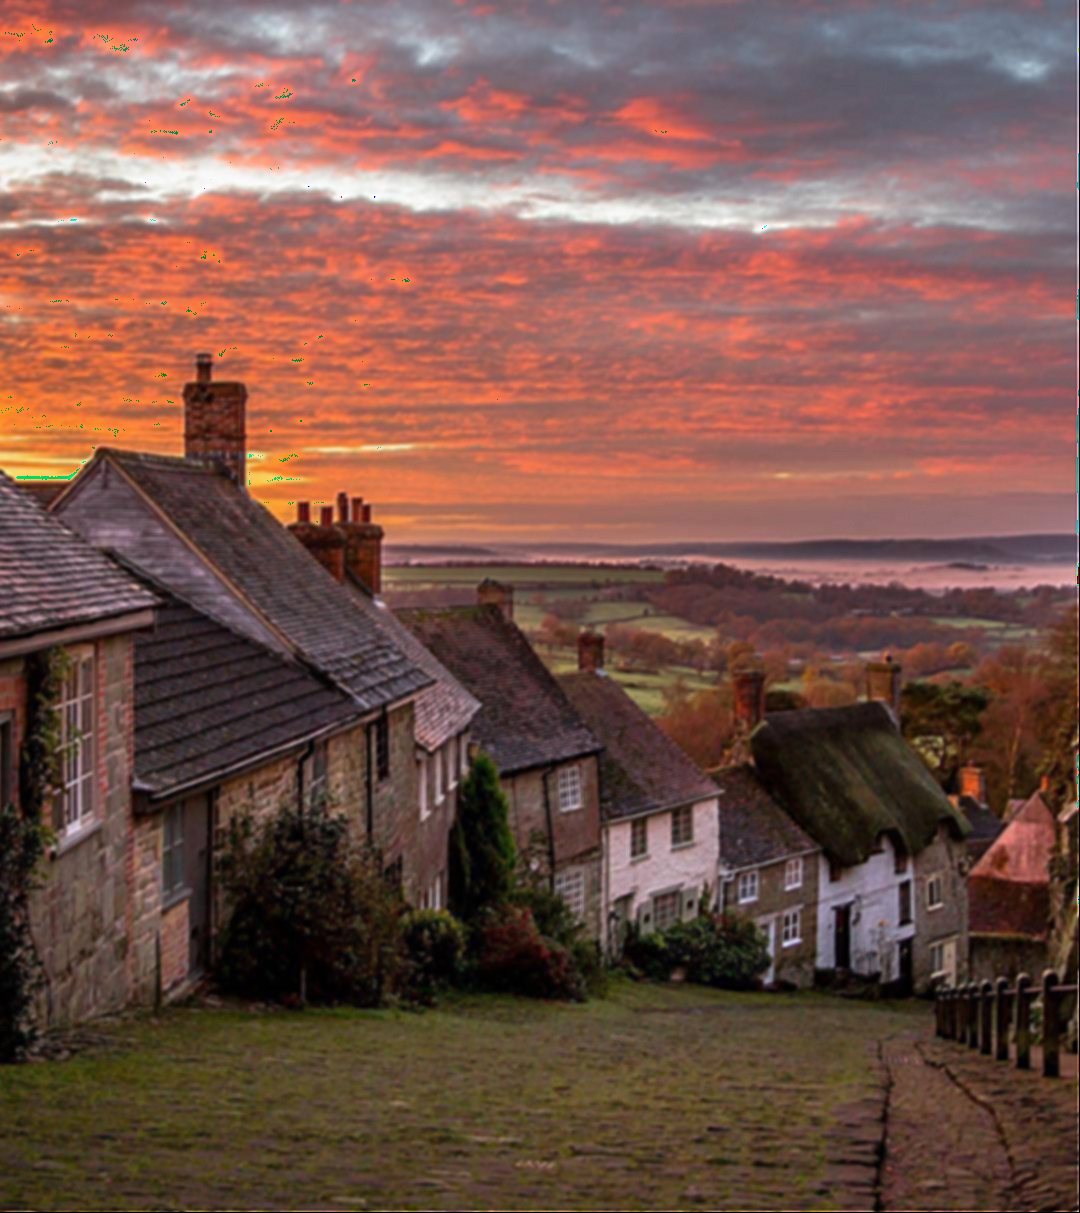
\includegraphics[width=1.6in]{figures/homes_deblur.png}
        \label{fig:hydra_deblur}}
    \end{center}
\end{figure*}

\end{document}
